%%%%%% a 18-array Affymetrix data %%%%%%%%%%%%%%%%%%
\newpage
\subsection{An Affymetrix experiment}
In this section we consider \Rfunction{abf1}, a 18 Affymetrix array
experiment. Data is from 3 mouse strains, three individuals per strain and
two arrays per individual. The experimental design is shown in Figure \ref{fig:abf1}.\\
\begin{figure}[htbp]
\centering
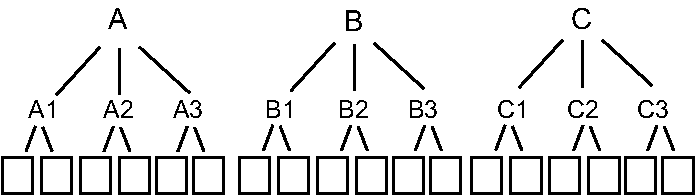
\includegraphics{abf1fig.pdf}
\caption{18-array Affymetrix experiment design}
\label{fig:abf1}
\end{figure}
{\bf Read Data} To reduce the size of {\em R/maanova} package, we do not
include .CEL files, thus you can not try following code. However this is the
typical example to read the data from {\em affy} package. Suppose you have .CEL
files and properly prepared TAB delimited text file under the working directory.
\begin{Sinput}
R> library(affy)
R> beforeRma <- ReadAffy()
R> rmaData <- rma(beforeRma)
R> datafile <- exprs(rmaData)
R> data1 <- read.madata(datafile=datafile,designfile="design.txt")
\end{Sinput}
You want to save the output of \Rfunction{exprs()} to avoid reading the .CEL file again.

Another \Rfunction{datafile} that {\em R/maanova} can read is a TAB delimited
text file.
\begin{Sinput}
R> data <- data.frame(probeid=row.names(datafile),datafile)
R> write.table(data,"data.dat",sep="\t",row=F,quote=F)
R> data2 <- read.madata(datafile="data.dat", designfile="design.txt", 
   probeid=1, intensity=2)
\end{Sinput}
{\bf {\tt Design File}} You must provide \Rfunction{designfile} information
according to the order in which {\em affy} package reads the .CEL files, and
save it as a TAB delimited text file. If you prepare \Rfunction{designfile} in advance, and want to read
the .CEL file according to the order of \Rfunction{designfile}, you need to
specify them at the \Rfunction{filename} in \Rfunction{ReadAffy()}. Here is the
an example script that one can prepare \Rfunction{designfile}.
\begin{Sinput}
R> design.table <- data.frame(Array=row.names(pData(beforeRma)))
R> write.table(design.table,"design.txt",sep="\t",row=F,quote=F) 
\end{Sinput}
You can find 'design.txt' file, containing 'Array' field under the working
directory. Open your favorite spread sheet and complete the rest of
information. In this example, 'Strain' and 'Sample' information are
provided. Table 1 shows the \Rfunction{designfile} of \Rfunction{abf1}. Note
that \Rfunction{abf1} has \Rfunction{Sample} column. \Rfunction{Sample} representing biological replicate is not a required
field in one color array, however it should be included in the \Rfunction{designfile}, when experiment has technical replicates.
\begin{table}[h]
\caption{Design file for \Rfunction{abf1}}
\begin{center}
\begin{tabular}{ccc}\hline
Array & Strain & Sample\\\hline
E111.CEL& AJ& 1\\
E112.CEL& AJ& 1\\
E113.CEL& AJ& 2\\
E114.CEL& AJ& 2\\
E115.CEL& B6& 3\\
E116.CEL& B6& 3\\
\ldots & \ldots & \ldots\\\hline
\end{tabular}\\
\end{center}
\end{table}

Another option to prepare \Rfunction{designfile} is making a {\tt data.frame}
(or {\tt matrix}) {\em R} object, and read it from {\em R} directly. This option is useful when the number of array is small. Again, make it sure that the information is provided by the order that \Rfunction{affy} reads the file.  
\begin{Sinput}
R> design.table <- data.frame(Array=row.names(pData(beforeRma)));
R> Strain <- rep(c('AJ', 'B6', 'B6xAJ'), each=6)
R> Sample <- rep(c(1:9), each=2)
R> designfile <- cbind(design.table, Strain, Sample)
R> abf1 <- read.madata(datafile, designfile=designfile)
\end{Sinput}
{\bf Model fitting} This data has technical replicates, and thus \Rfunction{Sample} is treated as \Rfunction{random} term. \Rfunction{residplot()} shows residual plot. 
\begin{Sinput}
R> data(abf1)
R> fit.full.mix <- fitmaanova(abf1, formula = ~Strain+Sample, 
   random = ~Sample)
R> resiplot(abf1, fit.full.mix)
\end{Sinput}
{\bf Test statistics} To test Strain effect in the model:
\begin{Sinput}
R> ftest.all = matest(abf1, fit.full.mix, test.method=c(1,1,0),
    shuffle.method="sample", term="Strain", n.perm= 100)
\end{Sinput}
If you are interested in the pairwise comparison, you can specify the contrast
matrix. Suppose you want to compare strain 1 vs. 2 and
strain 1 vs. 3. Then the corresponding contrast matrix should have 2 rows
(number of test) and three column (number of levels of
term). You may want to use \Rfunction{PairContrast()} to get all possible pairwise comparisons.  
\begin{Sinput}
R> C = matrix(c(1,-1,0,1,0,-1), ncol=3, byrow=T)
R> C.all = PairContrast(3)
R> ftest.pair = matest(abf1, fit.full.mix, Contrast = C, 
   term="Strain", n.perm=100)
\end{Sinput}
To derive FDR adjust p-value :
\begin{Sinput}
R> ftest.all = adjPval(ftest.all, method = 'jsFDR')
\end{Sinput}
{\bf Summarize the result} To get summary table, volcano plot and cluster :  
\begin{Sinput}
R> summarytable(ftest.all)
R> summarytable(ftest.all, method=c("Pvalperm"), test =c("Fs"), 
   whichTest=c("Fs.Pvalperm"), threshold=.1, outfile='shrotsummarytable.csv')

R> volcano(ftest.all)
R> idx.fix = volcano(ftest.pair)

R> cluster.kmean <- macluster(fit.full.mix, term="Strain",
   idx.gene=idx.fix$comparison1$idx.Fs,what="gene", method="kmean", 
   kmean.ngroups=5, n.perm=100)
R> con.kmean <- consensus(cluster.kmean, 0.7)
R> con.kmean$groupname
R> cluster.hc <- macluster(fit.full.mix, term="Strain",
   idx.gene=idx.fix$comparison1$idx.Fs,what="sample", method="hc", n.perm=100)
R> con.hc <- consensus(cluster.hc)
\end{Sinput}
Note that \Rfunction{ftest.pair} contains two comparisons, thus
\Rfunction{volcano(ftest.pair)} generates two plots. 